\section{Simulation results} 
To make the simulation results easier to understand, we outline a baseline model with one independent variable of interest and two covariates split by the different model sets. We then show the results of what happens when including more covariates, when the sample size increases or decreases, and having different correlations between the dependent variable and covariates. We will focus on results where the model is correctly specified. This means we will only focus on the model set with restrictions in this result section. However, in the \textit{Supplementary Information} accompanying this paper, what happens if one were to use models with no restrictions, i.e. including interactions without main effects. 

\subsection{Model specification}
Looking at the FPP and FPR between the different sets in the baseline model, it is clear that the highest FPP and FPR are obtained in the $x \times z$ and $x + z+ x \times z$ sets (see Figure \ref{fig:mainfigure1}). With the restriction that main effects must follow interactions, the FPP is 21.1\% for binary (dummy coded) variables and 18.1\% for continuous variables. \\ 
Looking at the FPR, we see that the proportion of models with a significant effect is around the expected 5\% when there are no interactions between the variable of interest and the covariates (see red bars in Figure \ref{fig:mainfigure1}). However, in the sets where there are interactions between the variable of interest and the covariates, the FPR increases to above 5\%. In this case, the FPR becomes higher than 10\% when the data is normally distributed. This means that over 10\% of all the models within this set had a significant main effect or interaction effect between a covariate and the variable of interest. 
 \\

% plot of the main analysis
\begin{figure}[hbt!]
%\figuretitle{Baseline model}
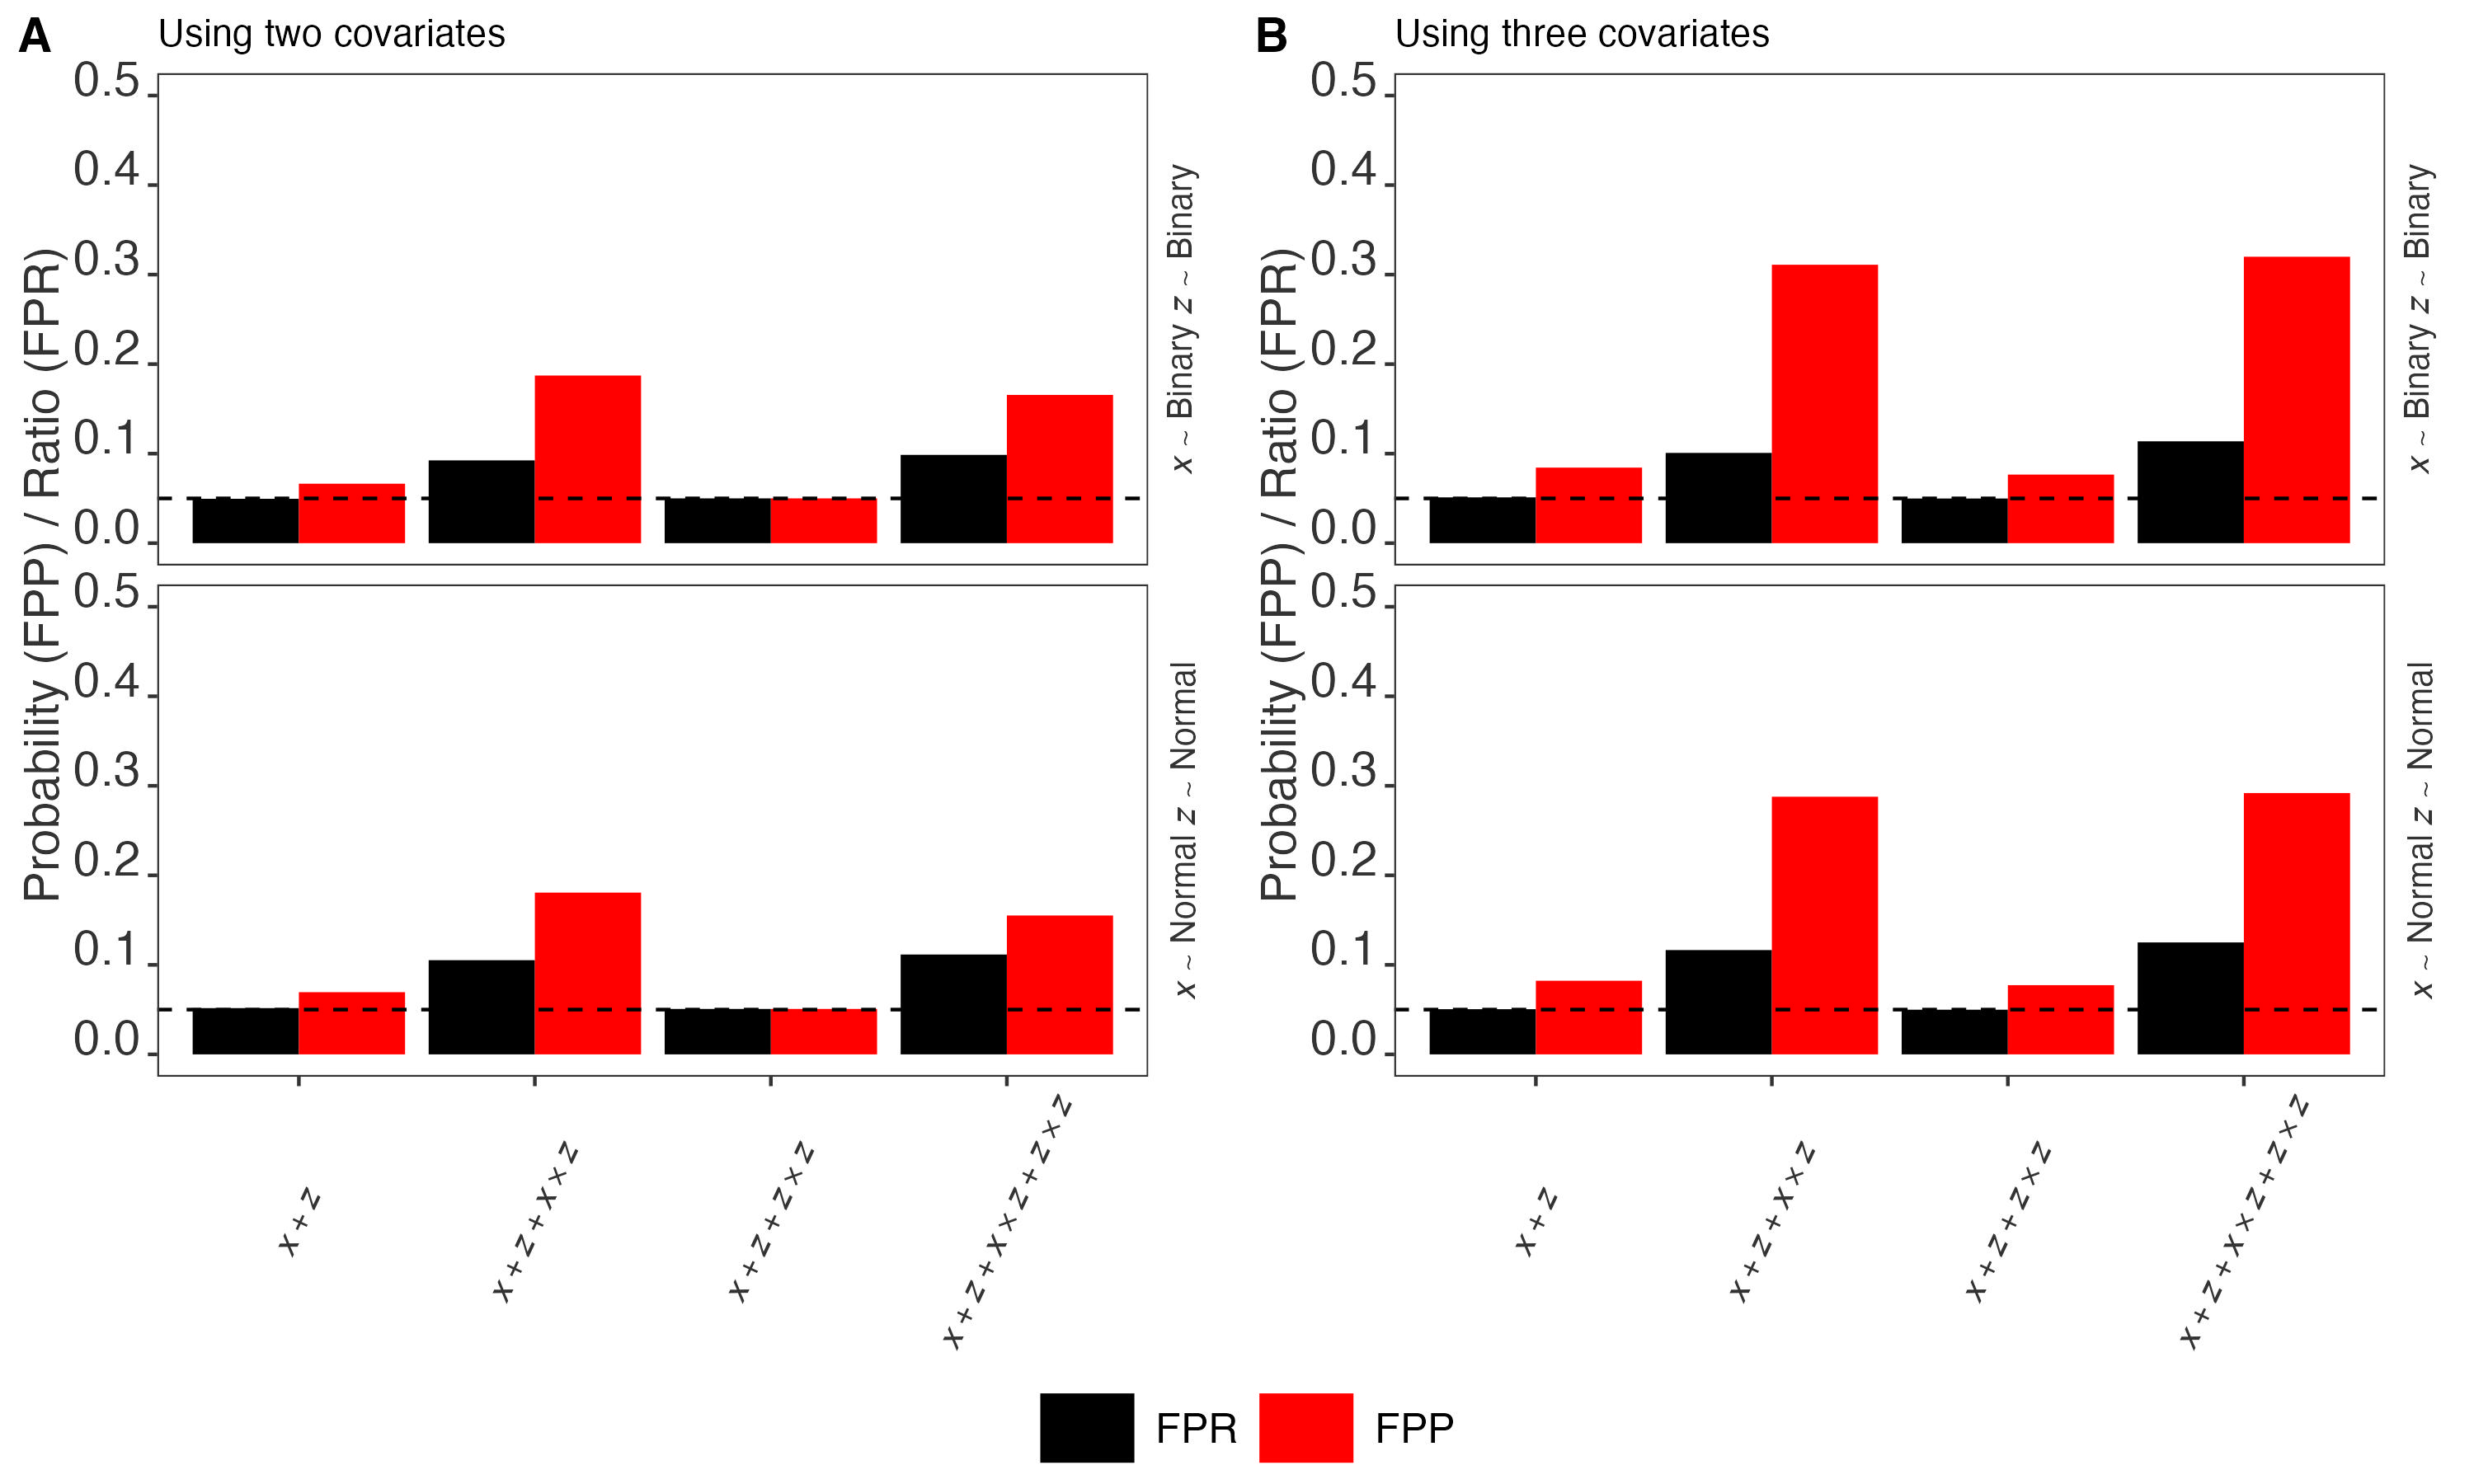
\includegraphics[width=0.6\textwidth]{R/Analysis/Result/Figures/Figure1_paper.jpeg}
\centering
\caption{The false-positive probability and false-positive ratio given different model sets, the presence of main effects when having interactions, and different distributions of the variable of interest and covariates. The sample size is set to 200, the correlation between the dependent variable and covariates is $r=0.2$. In plot A there is two covariates and in plot B there is used three covariates. The false-positive probability is shown in black, and the false-positive ratio is red. The dashed blacked line shows the critical value set at 0.05 }.
\label{fig:mainfigure1}
\end{figure}

\subsection{Number of covariates}
Adding one more covariate to the baseline model to get three in total increases the FPP across all model sets (see Figure \ref{fig:mainfigure2}).  The most significant increase in the FPP is in the $x + z+ x \times z + z \times z$ set, which increases by 14.7 percentage points when the variable of interest and covariates are binary (dummy coded) and 13.1 percentage points when the variables are continuous. This makes sense as the possible models here go from 3 to 58. Even in the sets that might be argued that are more reasonable and easier to argue for in a paper, such as the set $x + z+ x \times z $, the number of models goes from 5 to 19, and the FPP increases to around 30\% for both types of data. This increase is, however, also seen in the FPR, where the sets with interactions increase by a few percentage points. It is worth keeping in mind that if we expect the rejection rate to be 5\%, an increase of just a few percentage points can impact the interpretation of the results.  



\subsection{Sample size}
Increasing the sample size in the baseline model and thereby improving the estimates' precision has no effect in most of the conditions on either the FPP or FPR. This means that the higher accuracy in the analysis does not give any new information. Therefore, any argument that just because a sample is big implies it is better when it comes to false-positive does not make sense. The only case where more extensive samples should be valued is to safeguard against false negatives. It should be mentioned here that this result only holds when the analysis is done correctly (with restrictions on the model set); if this is not the case, an increase in the sample size can worsen the results. When there could be interactions without the main effect, the FPP and FPR can increase as the sample size becomes bigger. In that case, it is possible to more or less guarantee a false positive with a big enough sample (See \textit{Supplementary Information} for a complete set of results).


\subsection{Correlation between dependent variable and covariates}
Increasing the correlation between the dependent variable and covariates in the baseline model increases the FPP for all model sets (see Figure \ref{fig:appfigure1app} for a complete picture of the effect). When the correlation increases, then sets where there are interactions between the variable of interest and covariates, the FPP will increase the most. This effect is strongest for the set $x + z+ x \times z $. Here the FPP increases at around 4\% when the correlation goes from $r=0.2$ to $r=0.4$. The FPP also increases in the simpler model sets such as $x + z$. This means that the FPP is not only driven by the model set; the correlation between the covariates can also increase the FPP just by testing a set of models where it is known that the covariates would have a high correlation with the dependent variable. This is an important thing to remember when analysing as it is not only the number of variables that are collected that matters but also how they correlate with the dependent variable. 


\subsection{The need for correction}
In this part, we will examine why it is essential to correct the p-values when running a model with an interaction. As shown above, interactions are enough to increase both the FPP and FPR. Figure \ref{fig:mainfigure1_bon} shows the FPP and FPR when correcting the p-values using Bonferroni corrections \citep{dunn1961multiple}. This correction is performed by dividing the critical alpha by the number of model terms (main and interaction terms) containing the independent variable of interest. If, for instance, the variable of interest is present as main effect and with two interactions, the critical level is set to 1.66\% ($5/3$). This correction is enough to lower the FPR to the desired 5\%. The FPP is also lower; however, as the correction does not safeguard against multiple testing, the FPP is still higher than 5\%. To get an FPP of 5\%, the only solution is to perform one single analysis. The correction also works when having multiple covariates or using several dependent variables. (See the online \textit{Supplementary Information} for a complete set of results where the correction has been used)

\begin{figure}[hbt!]
%\figuretitle{Effect of increasing the number of covariates}
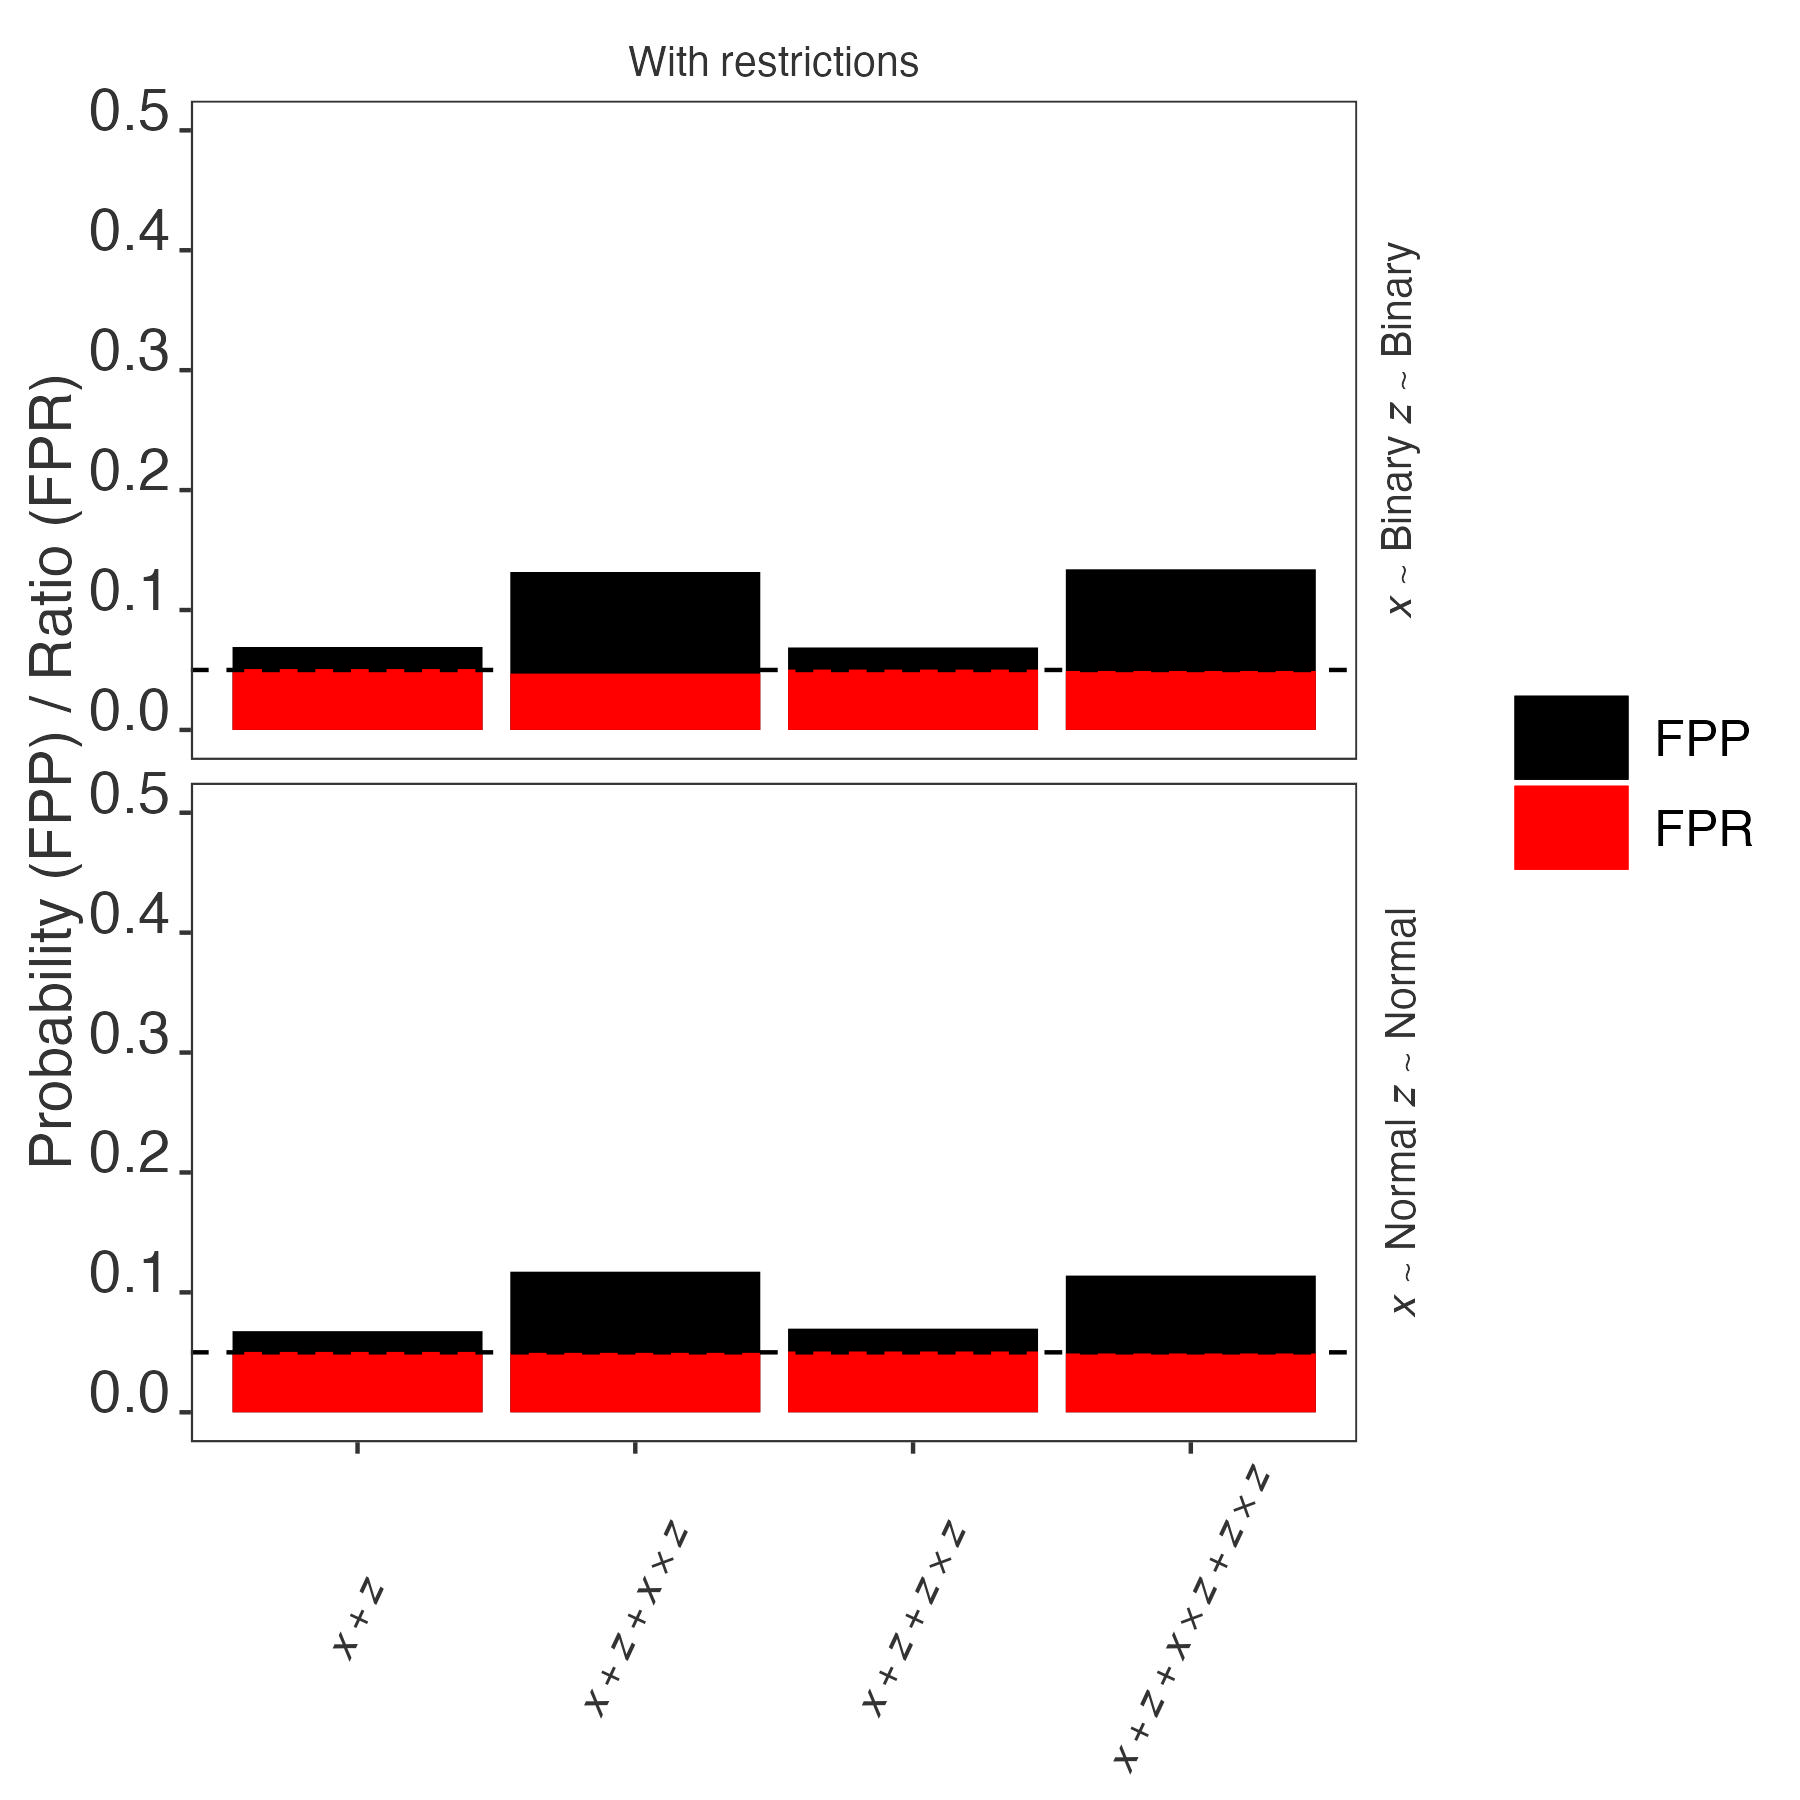
\includegraphics[width=0.6\textwidth]{R/Analysis/Result/Figures/Figure1ABon_with.jpeg}
\centering
\caption{The false-positive probability and false-positive ratio when using the baseline model but with Bonferroni correction. Black bars are the false-positive probability, and red denotes the false-positive ratio. The dashed blacked line shows the critical value, here set at 0.05.}
\label{fig:mainfigure1_bon}
\end{figure}

\subsection{Other results}
In the \textit{Supplementary Information}, an extensive set of other tests is being looked at. Here there is also looked at what happens when using several dependent variables (Figure \ref{fig:appfigure3} in the \textit{Supplementary Information}) and what happens when different outlier criteria are used (Figure \ref{fig:appfigure4} in the \textit{Supplementary Information}). In general, all these flexibilities increase the FPP to different degrees between the sets but do not seem to impact the FPR. What might be of more interest and, more important, is what happens when analysing model sets that have not been correctly specified. In this case, we mean having interactions but with no main effects. Doing this highly increases the FPP and FPR and, in some cases, guarantees a significant result as the FPR becomes close to 100 \% by just increasing the number of covariates, using higher correlated covariates with the dependent variable or increasing the sample size. This means that the papers that were identified should not be trusted.
